


\begin{frame}[fragile]{Just-In-Time Kernel Compilation}

 \begin{block}{Kernel Compilation}
   \begin{itemize}
    \item Library may provide hundreds of kernels
    \item Just-in-time compilation entails certain overhead
   \end{itemize}
 \end{block}

 \begin{block}{Little Experiment}
  \begin{itemize}
   \item Compile 64 trivial kernels of the form
   \begin{lstlisting}
__kernel void kernel_1_2(__global float *x){ x[1] = 2; }
   \end{lstlisting}
   \item Organize in 1 to 64 programs for 64 to 1 kernels each
  \end{itemize}
 \end{block}
 
\end{frame}




\begin{frame}{Just-In-Time Kernel Compilation}
\begin{center}
 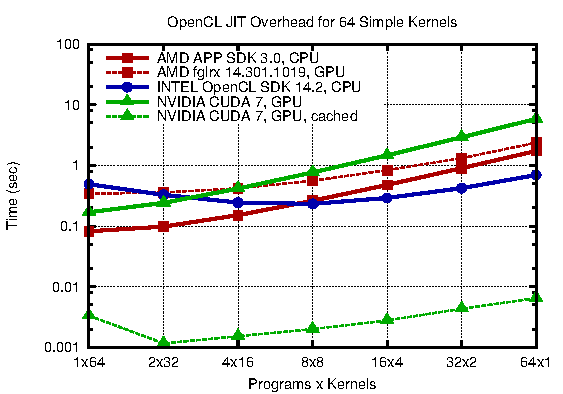
\includegraphics[width=0.95\textwidth]{figures/jit-overhead-5}
\end{center}
\end{frame}


\begin{frame}[fragile]{Just-In-Time Kernel Compilation}

 \begin{block}{OpenCL Program Cache}
   \begin{itemize}
    \item Compiled binaries stored in filesystem
    \item Implement in $\mathcal{O}(10)$ OpenCL SDKs?
    \item Implement in $\mathcal{O}(100)$ OpenCL-based libraries?
   \end{itemize}
 \end{block}

 \begin{block}{Proposed Solution}
   \begin{itemize}
    \item Make kernel caching a required (optional) feature for OpenCL SDKs
   \end{itemize}
 \end{block}

\end{frame}



\begin{frame}[fragile]{Just-In-Time Kernel Compilation}

 \begin{block}{SyCL to the Rescue?}
   \begin{itemize}
    \item SyCL compiler cannot generate binaries for all possible targets
    \item jit-overhead still an issue (unlike CUDA)
   \end{itemize}
 \end{block}

 \begin{block}{SPIR-V to the Rescue?}
   \begin{itemize}
    \item May reduce jit-compilation overhead substantially
    \item Broad availability required
   \end{itemize}
 \end{block}

\end{frame}
